%%%%%%%%%%%%%%%%%%%%%%%%%%%%%%%%%%%%%%%%%%%%%%%%%%%%%%%%%%%%%%%%%%%%%%%
% BAB 3
%%%%%%%%%%%%%%%%%%%%%%%%%%%%%%%%%%%%%%%%%%%%%%%%%%%%%%%%%%%%%%%%%%%%%%%

\mychapter{3}{BAB 3 LANDASAN KEPUSTAKAAN}

\section{Pengujian}

% kapan pengujian itu ada
% apa kekurangan dan kelebihan
% metode yang digunakan apa aja

Penggunaan perangkat lunak yang masif tanpa adanya standarisasi
membuat \emph{IEEE} merilis sebuah \emph{issue} pada November-December
1999. \emph{IEEE} dan \emph{ACM} kemudian membentuk tim gabungan untuk
mendefinisikan standardisasi pada proses pengembangan perangkat
lunak. Standardisasi tersebut memuat tentang \emph{scientific
  principles, engineering processes, standards, methods, tools,
  measurement and best practices}. Dimana pengujian atau
\emph{testing} termasuk di dalamnya
\parencite{burnstein2006practical}.

Pengujian bertujuan untuk menemukan cacat dan menguji kualitas suatu
perangkat lunak. Dalam proses pengujian terdapat beberapa metode,
tingkatan dan teknik. Setiap komponen pada bagian-bagian tersebut memiliki
kelemahan dan kekurangan tertentu. Proses testing juga akan
menghasilkan artefak-aretafak seperti \emph{test-scenario, test-case,
  test-data} dan \emph{test scripts} \parencite{burnstein2006practical}.

\subsection{Tahapan Pengujian}

Terdapat beberapa tahapan dalam pengujian. Tahapan-tahapan tersebut
seperti \emph{unit testing, integration testing, validation testing}
dan \emph{system testing} \parencite{presman2010software}. Pada
laporan ini tahapan yang akan dilakukan adalah \emph{unit} dan
\emph{integration}. Batasan tahapan pengujian tersebut ditentukan oleh
pembimbing lapangan dengan beberapa pertimbagan. Salah satunya adalah
waktu praktik kerja lapangan yang terbatas.

Tahapan awal dalam pengujian adalah pengujian \emph{unit}. Terdapat
beberapa pendapat berbeda mengenai \emph{'unit'} dalam \emph{unit
testing}. \textcite{martin2014unittest} berpendapat bahwa definisi
\emph{`unit'} dapat berarti \emph{single method, single class} maupun
kumpulan dari beberapa \emph{class}. \textcite{osherove2015art} tidak
mengikat definsi \emph{'unit'} pada \emph{class} maupun
\emph{method}. Melainkan mengikatnya dengan definsi atribut seperti
\emph{performance, reliability} dan \emph{consistency}. \emph{Google}
tidak menggunakan istilah \emph{unit, integration} ataupun
\emph{system} untuk merujuk pada tingkatan tertentu. Melainkan
menggunakan \emph{small, medium, large}
\parencite{whittaker2012google}. Sedangkan
\textcite{presman2010software} berpendapat bahwa fokus pengujian
\emph{unit} pada perangkat lunak konvensional adalah sebuah modul dan
fokus pengujian \emph{unit} pada perangkat lunak berorientasi objek
adalah \emph{class} dengan \emph{testable unit} terkecil adalah
\emph{operation} atau \emph{method}. Laporan ini mengikuti pendapat
\textcite{presman2010software} dalam pemahaman pengujian
\emph{unit}. Tahapan selanjutnya adalah \emph{Integration
testing}. \emph{Integrartion testing} merupakan pengujian yang
dilakukan pada kumpulan beberapa \emph{unit} yang telah diuji. Hal ini
dilakukan untuk memastikan suatu \emph{unit} akan berjalan dengan baik
jika dijalankan bersamaan dengan \emph{unit} yang lain. Meskipun
setiap \emph{unit} telah diuji secara individu, terdapat beberapa
kemungkinan galat yang terjadi ketika \emph{unit-unit} tersebut diuji
secara bersamaan. Beberapa kemungkinan galat yang akan terjadi
di antaranya adalah hilangnya data ketika melintasi \emph{interface}
dan komponen yang tidak berjalan semestinya ketika digabungkan
\parencite{presman2010software}. Pada proses pengujian \emph{unit} maupun
\emph{integrartion}, komponen tidak berupa \emph{stand-alone program}.
Maka dibutuhkan pembuatan \emph{stub} ataupun \emph{driver} selama proses pengujian.
\emph{Driver} hanyalah \emph{main program} tiruan yang menjalankan kasus uji.
Sedangkan \emph{stub} merupakan sebuah \emph{dummy subprogram} yang
bekerja menggantikan komponen-kompenen pengujuian yang
asli. Penggunaan \emph{stub} dapat digantikan dengan
\emph{mock}. Pembuatan \emph{mock} memiliki tujuan yang sama dengan
\emph{stub} \parencite{martin2007stub} .
Terlihat tahapan pengujian pada Gambar \ref{fig:testing-level}.

\begin{figure}[H]
  \centering
  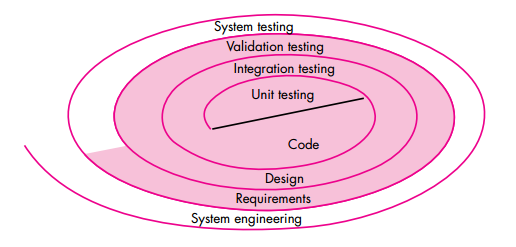
\includegraphics[width=.7\linewidth]{img/tahapan-pengujian}
  \caption{Tahapan Pengujian \parencite{presman2010software}}
  \label{fig:testing-level}
\end{figure}

\subsection{Metode Pengujian}

Metode atau yang juga dapat disebut \emph{point of view} merupakan
sudut pandang seorang \emph{tester} tatkala mendesain sebuah
\emph{test case}. Terdapat di antaranya \emph{white-box testing} dan
\emph{black-box testing}. Kedua metode tersebut memiliki kekurangan
masing-masing. Metode \emph{white-box testing} tidak dapat menemukan
kebutuhan yang belum diimplementasikan
\parencite{dijkstra1970notes}. Hal ini dapat diselesaikan dengan
penggunaan metode \emph{black-box testing}. Begitu juga dengan
kekurangan metode \emph{black-box testing} yang dapat menghasilkan
\emph{test-case} yang tidak tepat dan tidak dapat menemukan bagian
yang belum diuji \parencite{savenkov2008become}. Kelemahan pada metode
\emph{black-box testing} ini dapat diselesaikan dengan menggunakan
metode \emph{white-box testing}. Oleh karena itu, pada laporan ini
kedua metode tersebut digunakan.

\emph{White-box testing} merupakan suatu medote pengujian dimana
proses pengujiannya dilakukan dengan melihat internal perangkat lunak
sehingga pada tahapan ini seorang penguji wajib memiliki kemampuan
pemrograman. Pengujian ini dilakukan untuk menguji apakah \emph{logic}
dan \emph{data} pada perangkat lunak berfungsi sebagaimana mestinya
\parencite{myers2011art}. Di sisi lain \emph{black-box testing} hanya
menguji bagian luar suatu perangkat lunak. Pada tahapan ini
fungsionalitas suatu perangkat lunak diuji tanpa harus mengetahui
internalnya. Oleh karena itu, tidak dibutuhkan kemampuan pemrograman
saat membuat \emph{test case} pada pengujian \emph{black-box}. Penguji
hanya mengetahui bagaimana seharusnya perangkat lunak berjalan
(\emph{what}), bukan bagaimana perangkat lunak itu melakukan sesuatu
(\emph{how}). Pada tahapan ini penguji hanya mempertimbangkan masukan
(\emph{input}) dan keluaran (\emph{output}) perangkat lunak selama
mendesain \emph{test-case} \parencite{myers2011art}.


\subsection{Teknik Pengujian}

Terdapat beberapa teknik dalam pengujian. Pengujian semua \emph{path}
atau \emph{rigorous testing} pada proses \emph{white-box testing}
tidak mungkin dilakukan sehingga digunakan teknik \emph{basis path
testing} untuk menentukan \emph{path} yang akan diuji
\parencite{gregory2007path}. \emph{Rigorous testing} atau
\emph{exhaustive testing} (\emph{C$\infty$}) atau menguji semua
kemungkinan juga tidak mungkin dilakukan pada saat pengujian
\emph{black-box} sehingga penggunaan teknik \emph{equivalence
partitioning} untuk menentukan masukan yang \emph{valid} dan
\emph{invalid} diperlukan. Teknik \emph{boundary value analysis}
menjadi pelengkap teknik \emph{equivalence
partitioning}. \emph{Boundary value analysis} digunakan untuk
mendapatkan nilai masukan yang berada pada \emph{boundary} atau
\emph{corner}, karena nilai-nilai pada bagian tersebut memiliki
kemungkinan galat yang besar \parencite{presman2010software}.

\subsubsection{\emph{Basis Path Testing}}

\emph{Basis path testing} merupakan suatu teknik pengujian pada metode
\emph{white-box} yang diajukan oleh McCabe pada tahun 1996. Teknik ini
menggunakan penelitian McCabe yang sebelumnya yaitu \emph{cyclomatic
complexity} yang ia temukan pada 1976. Meski saat ini \emph{cyclomatic
complexity} banyak dikaitkan secara erat dengan rumus untuk menentukan
jumlah \emph{independent path}. \emph{Cyclomatic complexity} awalnya
ditemukan pada tahun 1976 diajukan untuk mengukur tingkat kompleksitas
suatu modul dalam sebuah program. Modul yang melebihi nilai
\emph{cyclomatic complexity} 10 direkomendasikan untuk dipisah atau
dilakukan \emph{refactoring}. Tujuan kedua dari rumus tersebut adalah
untuk melihat tingkat terstrukturnya (\emph{structuredness}) suatu
modul. Hal yang membuat \emph{cyclomatic complexity} dikaitkan secara
erat dengan proses \emph{basis path testing} karena kemdian McCabe
sadar bahwa \emph{cyclomatic complexity} dapat menemukan
\emph{independent path} pada suatu modul. \emph{Independent path} adalah
suatu jalur dalam sebuah program yang memperkenalkan setidaknya suatu rangkaian
pemrosesan baru atau kondisi baru. Hal tersebut yang
mengantarnya pada pengajuan \emph{basis path testing} pada 1996.
\emph{Basis path testing} memiliki keunggulan karena V(G) atau
\emph{vector space} memiliki nilai yang menjadi batas atas \emph{upper
bound} untuk membuat \emph{test-case} pada suatu program. Hal ini
menguntungkan penguji karena dapat menentukan ukuran batas selesainya
suatu pengujian. Selain itu, \emph{basis path testing} memiliki nilai
yang lebih baik dari pada \emph{branch coverage}, yaitu \emph{branch
coverage ≤ cyclomatic complexity ≤ all of paths}
\parencite{gregory2007path}.

Langkah-langkah pengujian \emph{basis path} adalah sebagai berikut
\parencite{presman2010software}:

\begin{enumerate}[
leftmargin=0pt, itemindent=20pt,
labelwidth=15pt, labelsep=5pt, listparindent=0.7cm,
align=left]
\item Membuat \emph{flow graph} dari desain atau \emph{code}.

  \emph{Flow graph} memiliki beberapa notasi seperti \emph{sequence,
    if, while, until} dan \emph{case}. Gambar notasi-notasi tersebut
  terlihat pada Gambar \ref{fig:notasi-flow-graph}. Terlihat \emph{flow graph}
  pada Gambar \ref{cfg:hallo} yang dihasilkan dari
  \emph{pseudocode} \ref{ps:hallo}

\item Menentukan \emph{cyclomatic complexity} dari \emph{flow graph}
  yang dihasilkan.

  \emph{Cyclomatic complexity} adalah suatu metrik perangkat lunak
  yang memberikan ukuran kuantitatif kompleksitas logis dari suatu
  program. \emph{Cyclomatic complexity} dapat ditentukan dengan menggunakan
  Rumus \ref{eq:perhitungan-cc}:

  \begin{equation}
    \begin{array}{l}
      V(G) = jumlah \thinspace region \\
      V(G) = E – N + 2 \\
      V(G) = P + 1, \thinspace dimana \thinspace P – predicate \thinspace node
    \end{array}
    \label{eq:perhitungan-cc}
  \end{equation}

  Maka Perhitungan \emph{cyclomatic complexity} yang dilakukan pada
  \emph{flow graph} \ref{cfg:hallo} menghasilkan
  nilai sebagai berikut:

  \begin{equation}
    \begin{array}{l}
      V(G) = 2 \thinspace regions \\
      V(G) = 4 \thinspace edges \thinspace – \thinspace 4 \thinspace
      nodes \thinspace + \thinspace 2 \thinspace = \thinspace 2 \\
      V(G) = 1 \thinspace predicate \thinspace node \thinspace +
      \thinspace 1 \thinspace = \thinspace 2
    \end{array}
    \label{eq:hasil-perhitungan-cc}
  \end{equation}

 Jadi, \emph{flow graph} pada Gambar \ref{cfg:hallo} memiliki nilai
 \emph{cyclomatic complexity} = 2.

\item Menentukan \emph{independent path}

  \emph{Independent path} adalah suatu jalur dalam sebuah program yang
  memperkenalkan setidaknya suatu rangkaian pemrosesan baru atau
  kondisi baru. Nilai dari V(G) memberikan batas atas dari banyaknya
  \emph{independent path} dari sebuah program. Dari contoh
  \emph{pseudocode} \emph{procedure hallo} kita mendapatkan 2 jalur
  \emph{independent} sebagai berikut : \par\null\par

  Jalur 1: 1 - 2 - 4 \par
  Jalur 2: 1 - 3 - 4

\item Membuat \emph{test case} yang akan menjalankan setiap jalur pada
  \emph{basis path}

  Terdapat dua \emph{test case} yang akan dihasilkan. Pertama
  \emph{test case} yang harus melewati jalur 1 sehingga pada \emph{test
    case} pertama nilai \emph{variable nama} harus bernilai
  \emph{true}. Pada \emph{test case} kedua nilai \emph{variable nama}
  harus bernilai \emph{false} agar jalur 2 dijalankan. \emph{Test case}
  yang dihasilkan tampak seperti pada Tabel
  \ref{tc:hallo}

\end{enumerate}

\begin{figure}[H]
  \centering
  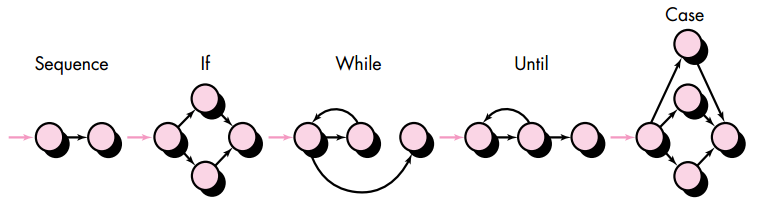
\includegraphics[width=.8\linewidth]{img/notasi-flow-graph}
  \caption{Notasi \emph{flow graph} \parencite{presman2010software}}
  \label{fig:notasi-flow-graph}
\end{figure}


\begin{center}
\begin{minipage}{0.8\textwidth}
\begin{code}
\begin{ignasicblock}[title=hallo,minted language=text]
procedure hallo(nama)
   IF nama == "Budi"          (1)
      RETURN "Hai" + nama     (2)
   ELSE
      RETURN "Nama kosong"    (3)
   ENDIF                      (4)
end
\end{ignasicblock}
\captionof{listing}{Contoh \emph{pseudocode}}
\label{ps:hallo}
\end{code}
\end{minipage}
\end{center}

\begin{figure}[H]
  \centering
  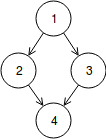
\includegraphics[width=.14\linewidth]{img/test-case/4node} % sama
  \caption{Representasi \emph{control flow graph} dari \emph{pseudocode} \ref{ps:hallo}}
  \label{cfg:hallo}
\end{figure}

\begin{longtable}{|P{.06\textwidth}|P{.30\textwidth}|P{.30\textwidth}|P{.10\textwidth}|P{.08\textwidth}|}
  \caption{\emph{Test case} dari contoh \emph{pseudocode} \ref{ps:hallo}} \label{tc:hallo}\\
  \hline
  \textbf{Jalur} & \textbf{Prosedur Uji} & \textbf{\emph{Expected Result}} \\\hline
  %
  1 & Memberikan nilai \emph{``Budi''} pada variable \emph{nama} &
                                                                   Program menampilkan ``Hai Budi'' \\\hline
                                                                   %
  2 & Tidak memberikan nilai apapun pada variable \emph{nama} &
                                                                   Program menampilkan ``Nama kosong'' \\\hline
  %

\end{longtable}


\subsubsection{Equivalence Partitioning}

\emph{Equivalence partitioning} merupakan suatu teknik dalam metode
pengujian \emph{black-box} dimana prosesnya adalah membangi masukan
kepada kelas-kelas data. Dari kelas-kelas tersebut \emph{test case}
nantinya didapatkan. \emph{Equivalence class} merepresentasikan
keadaan valid tau tidak validnya suatu masukan. Beberapa kondisi
masukan di antaranya \emph{numeric value, range of values, set of
related values,} atau \emph{boolean condition}. \emph{Equivalence
partitioning} dapat di definisikan sesuai dengan panduan berikut
\parencite{presman2010software}:

\begin{enumerate}[
leftmargin=0pt, itemindent=20pt,
labelwidth=15pt, labelsep=5pt, listparindent=0.7cm,
align=left]

\item Jika kondisi masukan adalah \emph{range}. Makan satu valid dan
  dua invalid \emph{equivalence class} di definisikan.
\item Jika kondisi masukan adalah \emph{specific value}. Makan satu valid dan
  dua invalid \emph{equivalence class} di definisikan.
\item Jika kondisi masukan adalah \emph{member of a set}. Makan satu valid dan
  satu invalid \emph{equivalence class} di definisikan.
\item Jika kondisi masukan adalah \emph{boolean}. Makan satu valid dan
  satu invalid \emph{equivalence class} di definisikan.

\end{enumerate}

\newpage

Jika data masukan bertipe \emph{range} dan masukan yang valid adalah
\emph{range} bernilai 4 hingga 10. Maka masukan yang tidak valid
adalah semua angka yang kurang dari 4 dan semua angka yang lebih dari
10 seperti terlihat pada Gambar \ref{fig:contoh-ep-marked}. Data
yang digunakan untuk \emph{test case} pada tipe masukan \emph{range}
berjumlah 3. Satu bernilai valid dan dua bernilai invalid. Oleh karena itu,
data masukan \emph{valid} yang kita gunakan adalah 11 dan 7. Sedangkan
data \emph{invalid} yang digunakan adalah 3.

\begin{figure}[H]
  \centering
  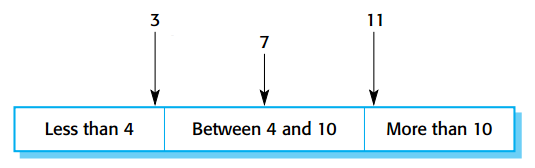
\includegraphics[width=.6\linewidth]{img/contoh-ep-marked}
  \caption{Contoh \emph{equivalence partitioning} \parencite{sommerville2014software}}
  \label{fig:contoh-ep-marked}
\end{figure}

\subsubsection{\emph{Boundary Value Analysis}}

\emph{Boundary value analysis} merupakan suatu teknik yang melengkapi
\emph{equivalence partitioning}. \emph{Boundary value analysis}
dikembangkan untuk menganalisis nilai yang berada pada \emph{boundary}
masukan, karena nilai pada \emph{boundary} atau \emph{corner} memiliki
peluang galat yang lebih tinggi. \emph{Boundary value analysis} tidak
berdiri sendiri, melainkan merupakan teknik yang melengkapi
\emph{equivalence partitioning}. Maka \emph{boundary value analysis}
mengambil nilai yang bersifat ``pojok'' dari nilai hasil
\emph{equivalence partitioning}. Panduan pemilihan nilai
\emph{boundary value analysis} di antaranya sebagai berikut
\parencite{presman2010software}:

\begin{enumerate}[
leftmargin=0pt, itemindent=20pt,
labelwidth=15pt, labelsep=5pt, listparindent=0.7cm,
align=left]

\item Jika masukan merupakan sebuah \emph{range} dari a hingga
  b. Maka nilai yang digunakan untuk \emph{test case} adalah satu
  nilai di atas a dan satu nilai di bawah b.
\item Jika masukan merupakan sebuah \emph{number of values}. Maka
  nilai yang digunakan untuk \emph{test case} adalah nilai maksimum
  dan minimum serta satu nilai di atas maksimum dan satu nilai di
  bawah minimum.
\end{enumerate}

Jika data masukan bertipe \emph{range} dari 4 hingga 10. Maka nilai
yang didapatkan untuk pengujian adalah nilai maksimum dan minimum
serta satu nilai di atas maksimum dan satu nilai di atas minimum. Jadi
nilai yang didapatkan adalah 4, 10, 3, dan 11 seperti terlihat pada
Gambar \ref{fig:contoh-bva-marked}.

\begin{figure}[H]
  \centering
  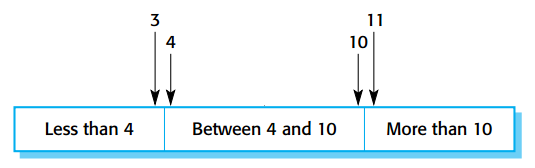
\includegraphics[width=.6\linewidth]{img/contoh-bva-marked}
  \caption{Contoh \emph{boundary value analysis} \parencite{sommerville2014software}}
  \label{fig:contoh-bva-marked}
\end{figure}

\subsection{\emph{Automated Testing}}

Menjalankan semua \emph{test case} secara manual sangat menyita
waktu. Bahkan mereka dapat menyita 50\% dari pada waktu pengembangan
\parencite{brooks1995mythical}. \emph{Automated testing} dapat
digunakan untuk mempercepat proses pengujian. \emph{Automated testing}
adalah proses menjalakan \emph{test case} secara otomatis.
\emph{Automated testing} berjalan dengan adanya \emph{trigger}. Baik
dalam bentuk \emph{event} maupun \emph{time}. Prosesnya adalah dengan
menjalankan \emph{test case} dan membandingkannya dengan \emph{output}
yang sudah ditentukan. Hasil perbandingan tersebut akan dilaporkan
kepada penguji secara otomatis setelah \emph{automated testing}
selesai dijalankan \parencite{marcellintravis}. \emph{Automated
  testing} dibangun dengan menggunakan \emph{script} sesuai dengan
\emph{test case} yang didapatkan dari tahapan pengujian
\emph{white-box} maupun \emph{black-box}. Tampak pada Tabel Kode
\ref{ts:hallo} merupakan \emph{script} yang dibangun untuk melakukan
pengujian secara otomatis. \emph{Script} tersebut didapatkan dari
\emph{test case} untuk pengujian \emph{pseudocode hallo} pada Tabel
Kode \ref{tc:hallo}. \emph{Script} ini nantinya dijalankan dengan
kakas bantu \emph{pytest} untuk melakukan pengecekan berhasil atau
gagalnya suatu pengujian secara otomatis. Sedangkan \emph{trigger} untuk
menjalankan \emph{pytest} secara otomatis dilakukan dengan bantuan
kakas bantu \emph{travis-ci}.

\begin{center}
\begin{minipage}{0.8\textwidth}
\begin{code}
\begin{ignasicblock}[title=test\_hallo,minted language=Python]
      def test_case_1():
          assert hallo("Budi") == "Hai Budi"

      def test_case_2():
          assert hallo("Ani") == "Nama Kosong"
\end{ignasicblock}
\captionof{listing}{\emph{Contoh script atomated testing}}
\label{ts:hallo}
\end{code}
\end{minipage}
\end{center}


\section{NEO-CLI}

\emph{Neo-cli} merupakan sebuah perangkat lunak orkestrasi untuk
infrastruktur \emph{cloud}. Sifatanya yang \emph{agnostic} dapat
melakukan orkestrasi kepada berbagai \emph{cloud platform} seperti
\emph{OpenStack} maupun \emph{Amazon Web Services}. \emph{Neo-cli}
dikembangkan dengan \emph{Python} dan beberapa \emph{depedency}
lainnya seperti \emph{GitPython, ncurses} dan lainnya
\parencite{neo-cli-ol}. Kedepannya \emph{neo-cli} akan mendukung
penggunakan \emph{query languange} bernama \emph{BQL}
\parencite{irawanbiznet}.

\section{Teknologi Pengujian Perangkat Lunak}

\subsection{Pytest}

\emph{Python} memiliki \emph{built-in library} untuk melakukan
pengujian bernama \emph{python unittest}. Tetapi \emph{python
  unittest} memiliki banyak kekurangan, salah satunya adalah kurangnya
fungsionalitas yang dimiliki untuk melakukan pengujian. Oleh karena
itu, penggunaan \emph{pytest} diutamakan \emph{knupp}.  \emph{Pytest}
dibangun pada tahun 2014 oleh Holger Krekel. Kerkel membangun seluruh
\emph{code base} \emph{pytest} dengan \emph{python}
\parencite{pytest-ol}. Pada laporan ini, \emph{pytest} digunakan untuk
menjalankan \emph{test case} dan mengecek apakah suatu pengujian
berhasil atau gagal. Contoh pengujian yang dilakukan dari Tabel Kode
\ref{ts:hallo} akan terlihat seperti Gambar
\ref{fig:pytest-berhasil} jika berhasil dan akan terlihat seperti
Gambar \ref{fig:pytest-gagal} jika gagal. Pengujian gagal karena \emph{variable nama}
diganti nilainya menjadi selain ``budi''.

\begin{figure}[H]
  \centering
  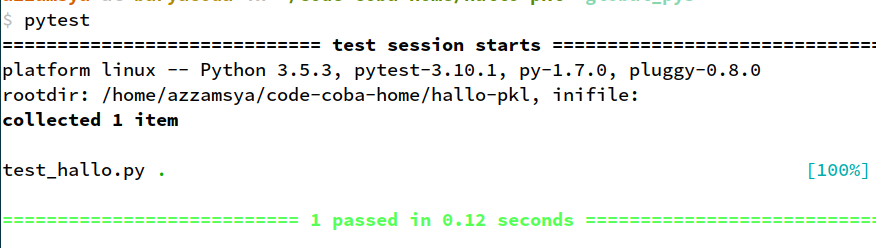
\includegraphics[width=.7\linewidth]{img/pytest-berhasil}
  \caption{Pengujian berhasil}
  \label{fig:pytest-berhasil}
\end{figure}

\begin{figure}[H]
  \centering
  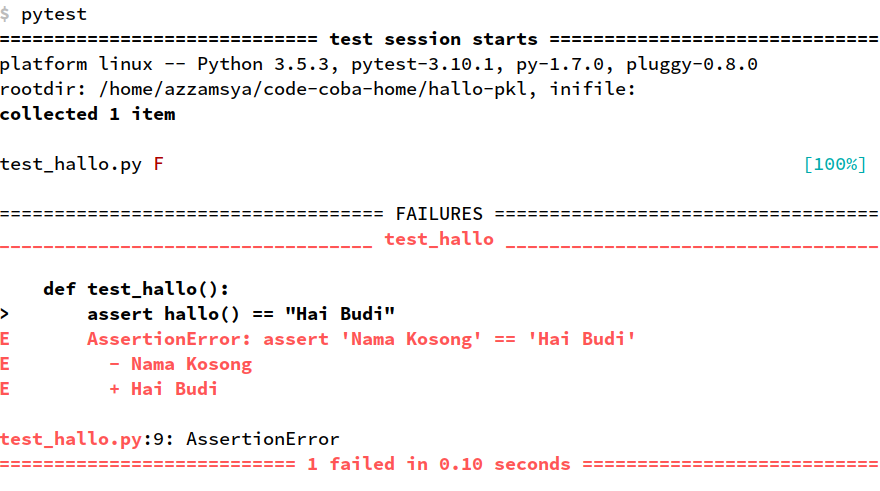
\includegraphics[width=.7\linewidth]{img/pytest-gagal}
  \caption{Pengujian gagal}
  \label{fig:pytest-gagal}
\end{figure}


\subsection{Coverage.py}

\emph{Coverage.py} merupakan kakas bantu yang digunakan untuk
menghitung tingkat cakupan (\emph{coverage}) suatu
pengujian. \emph{Coverage.py} memiliki fitur untuk mengekspor hasil
\emph{coverage} dalam bentuk \emph{Text, HTML, PDF} maupun
\emph{XML}. Ned Batchelder menciptakan \emph{coverage.py} pada 2004
dan merilisnya dengan lisensi \emph{Apache 2.0}
\parencite{coverage-ol}. Pada laporan ini \emph{coverage.py} digunakan
untuk menghitung seberapa besar cakupan pengujian yang telah
dilakukan. Terlihat pada Gambar \ref{fig:cov-1} cakupan pengujian
hanya mencapai 80\%, jika pengujian hanya menjalankan \emph{test case}
pertama. Cakupan akan mencapai 100\% ketika menjalankan semua
\emph{test case} pada \emph{test script} \ref{ts:hallo}.
Terlihat pada Gambar \ref{fig:cov-2} cakupan mencapai 100\% tatkala semua
\emph{test case} dijalankan.

\begin{figure}[H]
  \centering
  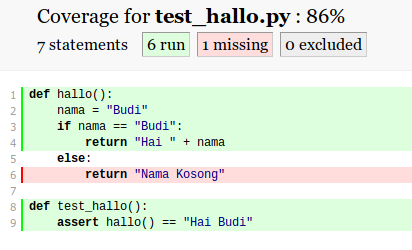
\includegraphics[width=.5\linewidth]{img/cov-1}
  \caption{86\% \emph{coverage}}
  \label{fig:cov-1}
\end{figure}

\begin{figure}[H]
  \centering
  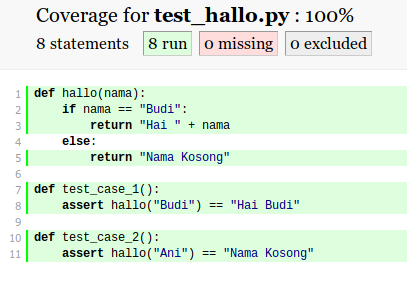
\includegraphics[width=.5\linewidth]{img/cov-2}
  \caption{100\% \emph{coverage}}
  \label{fig:cov-2}
\end{figure}


\subsection{Travis CI}

\begin{figure}[H]
  \centering
  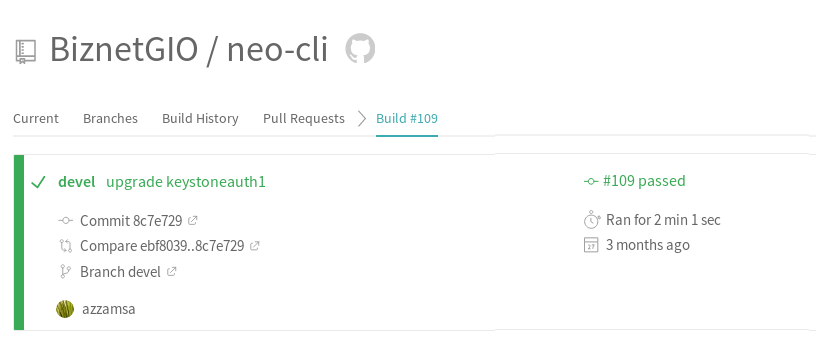
\includegraphics[width=.8\linewidth]{img/travis-head}
  \caption{\emph{Travis-ci} melaporan status pengujian}
  \label{fig:travis-head}
\end{figure}

\emph{Travis CI} merupakan sebuah kakas bantu yang dapat mengatur
\emph{trigger} dalam proses \emph{automated test}.  \emph{Travis CI}
mendukung banyak bahasa pemrograman seperti \emph{Python, C++, Ruby}
dan lainnya. Semua pengaturan pada \emph{travis ci} diatur dengan
format \emph{YAML} dalam berkas `\emph{.travis.yml}'. Pengecekan juga
dapat dilakukan secara otomatis pada \emph{branch} maupun \emph{pull
  request}. Hasilnya dapat dikirimkan melalui \emph{web notification}
maupun surel. \emph{Travis ci} dibangun di Jerman pada 2011 oleh
Travis CI, GmbH. \emph{Travis ci} dirilis dengan lisensi \emph{MIT}
\parencite{travis-ol}. Di dalam laporan ini, \emph{travis-ci}
digunakan untuk mengatur \emph{trigger} dalam proses \emph{automated
  testing}. Pengujian nantinya akan dijalankan secara otomatis oleh
\emph{travis-ci} pada \emph{trigger-trigger} tertentu yang telah
ditentukan. \emph{Trigger} dapat berbentuk waktu seperti hari atau
jam. Maupun berbentuk \emph{event} seperti dijalankan ketika terdapat
perubahan \emph{code}. Tampak pada Gambar \ref{fig:travis-head}
\emph{travis-ci} melaporkan bahwa pengujian yang dijalankan secara
otomatis pada \emph{event} \emph{commit upgrade keystoneauth1} berjalan
dengan sukses dan memakan waktu dua menit.


%%% Local Variables:
%%% mode: latex
%%% TeX-master: "pkl"
%%% End:
